\subsection{Subprocesso de Verificação e Validação}

Relembrando que o proposito da verificação é confirmar que cada serviço e/ou produto de trabalho do processo ou do
projeto atende apropriadamente os requisitos especificados \cite{pressman1} e validação tem como objetivo validar que um
produto de software atenderá a seu objetivo quando colocado no ambiente para o qual foi desenvolvido \cite{sommerville}

\begin{figure}[h!]
	\centering
  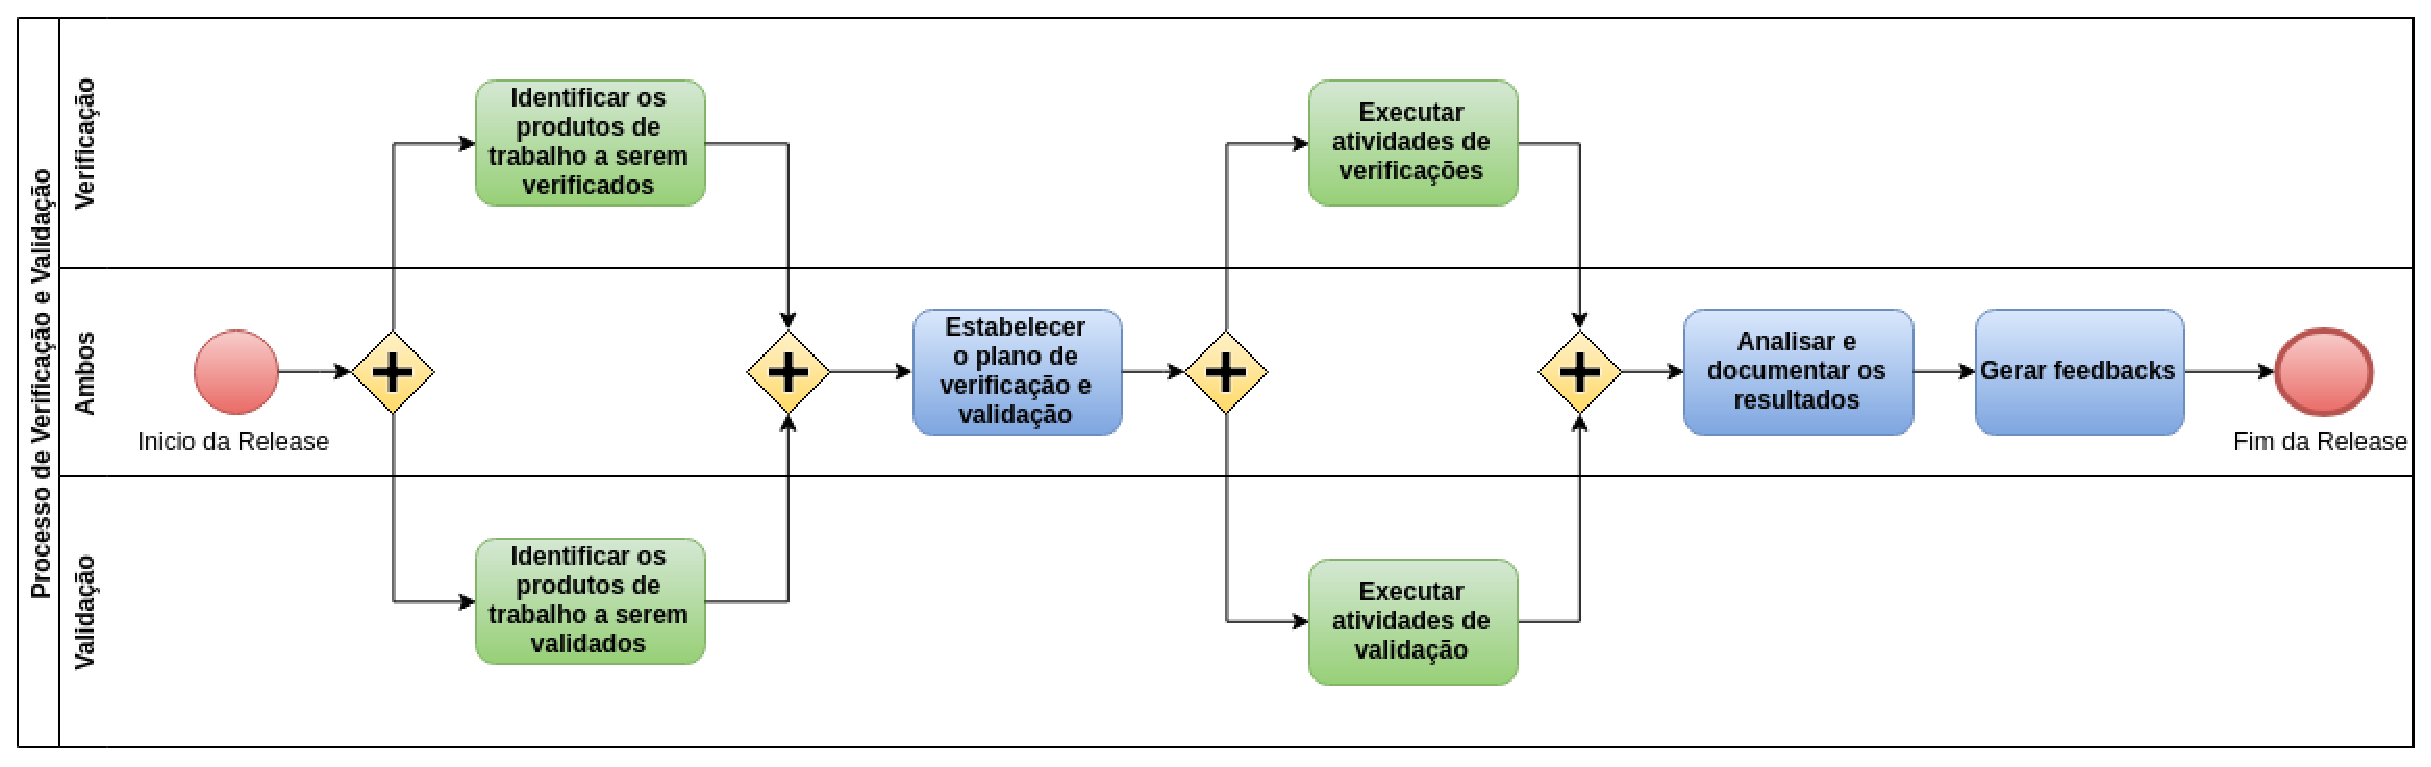
\includegraphics[keepaspectratio=true,scale=0.35]{figuras/VeV.eps}
  \caption[Subprocesso de Verificação e Validação.]{Subprocesso de Verificação e Validação. Fonte: Autor}
	\label{fig:vev}
\end{figure}

\begin{itemize}
  \item \textbf{Identificar os produtos de trabalho}:
  \begin{itemize}
    \item \textbf{Descrição}: Análisar os produtos de trabalho que serão produzidos na release e selecionar
      aqueles que serão verificados e/ou validados (documentos e códigos)
    \item \textbf{Entradas}: N/A
    \item \textbf{Saídas}: Lista de produto de trabalhos (documentos e códigos)
  \end{itemize}
  \item \textbf{Estabelecer o plano de verificação e validação}:
  \begin{itemize}
    \item \textbf{Descrição}: Criar ou Consultar o plano de verificação e validação para selecionar uma técnica apropriado
    para sua execução, sendo ela estática ou dinâmica.
    \item \textbf{Entradas}: Plano de verificação e validação se houver
    \item \textbf{Saídas}: Plano de verificação e validação caso não houver.
  \end{itemize}
  \item \textbf{Executar atividades de verificação e validação}:
  \begin{itemize}
    \item \textbf{Descrição}: Nas documentações será utilizado a técnica de Peer Review, porém com um único membro
      que terá como objetivo revisar toda a documentação a fim de encontrar erros ou verificar se algo precisa ser
      atualizado. Na parte de código a técnica que será utilizada são testes unitários, integração e de aceitação
      automatizados.
    \item \textbf{Entradas}: Plano de verificação e validação com a descrição das respectivas técnicas
    \item \textbf{Saídas}: Tabela com os documentos que precisam ser melhorados e novas issues de bugs encontrados.
  \end{itemize}
  \item \textbf{Análisar e Documentar os resultados}:
  \begin{itemize}
    \item \textbf{Descrição}: Ao final de cada sprint será documentado no resultado da sprint os documentos que necessitam
    ser atualizados e melhados. e Será criado issues para as dívidas técnicas encontradas.
    \item \textbf{Entradas}: Tabela com os documentos que precisam ser melhorados e novas issues de bugs encontrados.
    \item \textbf{Saídas}: Resultado da sprint com os resultados do processo de VeV.
  \end{itemize}
  \item \textbf{Gerar Feedbacks}:
  \begin{itemize}
    \item \textbf{Descrição}: Gerar feedbacks para que os artefatos possam ser atualizados e melhorados por meio do
    resultado da sprint.
    \item \textbf{Entradas}: Resultado da sprint com os resultados do processo de VeV
    \item \textbf{Saídas}: Feedbacks para a próxima sprint.
  \end{itemize}
\end{itemize}
